% Document
\documentclass[fontsize=8pt,paper=a4,paper=landscape,DIV=calc,]{scrartcl}
\usepackage[T1]{fontenc}
\usepackage{noto}
\usepackage[nswissgerman,english]{babel}
\renewcommand{\familydefault}{\sfdefault}

% Format
\usepackage[top=5mm,bottom=1mm,left=5mm,right=5mm,includehead]{geometry}
\setlength{\headheight}{\baselineskip}
\setlength{\headsep}{0mm}

\usepackage{multicol}
\setlength{\columnsep}{2mm}
\setlength{\columnseprule}{0.1pt}

% Color
\usepackage[svgnames]{xcolor}

% Math
\usepackage{amsmath}
\usepackage{amssymb}
\usepackage{amsfonts}
\newcommand*{\eq}{=}

%% Venn Diagrams
\usepackage{venndiagram}

%% Trees
%%% https://tex.stackexchange.com/a/425271
\usepackage{forest}
\forestset{
    ptree/.style={
        for tree={
            % grow'=0,
            % parent anchor=children,
            % child anchor=parent,
            grow'=east,
            parent anchor=east,
            child anchor=west,
            text width=7mm
        },
        before typesetting nodes={
            for tree={
                split option={content}{:}{content, my edge label},
            },
        },
    },
    my edge label/.style={
        if={
            > O_= {n'}{1}
        }{
            edge label={node [midway, below left, font=\tiny] {#1} }
        }{
            edge label={node [midway, above left, font=\tiny] {#1} }
        },
    }
}

% Standards
\newcommand{\rfc}[1]{\href{https://www.rfc-editor.org/rfc/rfc#1.html}{RFC#1}}
\newcommand{\ieee}[1]{\href{https://ieeexplore.ieee.org/search/searchresult.jsp?queryText=#1}{IEEExplore #1}}

% Code
\usepackage{listings}

\lstset{
   extendedchars=true,
   basicstyle=\footnotesize\ttfamily,
   tabsize=2,
   breaklines=true,
   showspaces=false,
   showtabs=false
   showstringspaces=false,
}

%% https://tex.stackexchange.com/a/536018
%% Allow for German characters in lstlistings.
\lstset{literate=
    {Ö}{{\"O}}1
    {Ä}{{\"A}}1
    {Ü}{{\"U}}1
    {ü}{{\"u}}1
    {ä}{{\"a}}1
    {ö}{{\"o}}1
}

%% Java Language definition
\lstdefinelanguage{java}{
  keywords=[1]{abstract, assert, boolean, byte, char, class, default, double,
  enum, extends, final, float, implements, import, instanceof, int, interface,
  long, native, null, package, private, protected, public, short, static,
  strictfp, super, synchronized, this, throw, throws, transient, void,
  volatile},
  keywordstyle=[1]\color{DarkBlue}\bfseries,
  keywords=[2]{if, else, while, do, try, case, catch, finally, new, break,
  continue, return, switch},
  keywordstyle=[2]\color{DarkRed}\bfseries,
  identifierstyle=\ttfamily,
  sensitive=false,
  comment=[l]{//},
  morecomment=[s]{/*}{*/},
  commentstyle=\color{DarkGray},
  stringstyle=\color{DarkGreen},
  morestring=[b]',
  morestring=[b]"
}

% Images
\usepackage{graphicx}
\graphicspath{{graphic/}}

% Links
\usepackage{hyperref}
\hypersetup{
    colorlinks=true,
    linkcolor=blue,
    filecolor=magenta,
    urlcolor=cyan,
}

% Smaller Lists
\usepackage{enumitem}
\setlist[itemize,enumerate]{leftmargin=3mm, labelindent=0mm, labelwidth=1mm, labelsep=1mm, nosep}
\setlist[description]{leftmargin=0mm, nosep}
\setlength{\parindent}{0cm}

% Smaller Titles
\usepackage[explicit]{titlesec}

%% Color Boxes
\newcommand{\sectioncolor}[1]{\colorbox{black!60}{\parbox{0.97\linewidth}{\color{white}#1}}}
\newcommand{\subsectioncolor}[1]{\colorbox{black!50}{\parbox{0.97\linewidth}{\color{white}#1}}}
\newcommand{\subsubsectioncolor}[1]{\colorbox{black!40}{\parbox{0.97\linewidth}{\color{white}#1}}}
\newcommand{\paragraphcolor}[1]{\colorbox{black!30}{\parbox{0.97\linewidth}{\color{white}#1}}}
\newcommand{\subparagraphcolor}[1]{\colorbox{black!20}{\parbox{0.97\linewidth}{\color{white}#1}}}

%% Title Format
\titleformat{\section}{\vspace{0.5mm}\bfseries}{}{0mm}{\sectioncolor{\thesection~#1}}[{\vspace{0.5mm}}]
\titleformat{\subsection}{\vspace{0.5mm}\bfseries}{}{0mm}{\subsectioncolor{\thesubsection~#1}}[{\vspace{0.5mm}}]
\titleformat{\subsubsection}{\vspace{0.5mm}\bfseries}{}{0mm}{\subsubsectioncolor{\thesubsubsection~#1}}[{\vspace{0.5mm}}]
\titleformat{\paragraph}{\vspace{0.5mm}\bfseries}{}{0mm}{\paragraphcolor{\theparagraph~#1}}[{\vspace{0.5mm}}]
\titleformat{\subparagraph}{\vspace{0.5mm}\bfseries}{}{0mm}{\subparagraphcolor{\thesubparagraph~#1}}[{\vspace{0.5mm}}]

%% Title Spacing
\titlespacing{\section}{0mm}{0mm}{0mm}
\titlespacing{\subsection}{0mm}{0mm}{0mm}
\titlespacing{\subsubsection}{0mm}{0mm}{0mm}
\titlespacing{\paragraph}{0mm}{0mm}{0mm}
\titlespacing{\subparagraph}{0mm}{0mm}{0mm}

%define header and footer
\usepackage{fancyhdr}
\pagestyle{fancy}

\fancyhead[RO]{\AUTHOR\hspace{4pt}|\hspace{4pt}\INSTITUTE}
\fancyhead[LO]{\TITLE}
\usepackage[style=iso]{datetime2}
\fancyfoot[RO]{\today}
\renewcommand\headrulewidth{0pt}
\renewcommand\footrulewidth{0pt}
\headsep = -2pt
\footskip = 0pt

% no vertical distribution
%% explanation: we copy the macro columnbreak to stdcolumnbreak
%% we now redefine columnbreak to always fill up null space and then execute the standard columnbreak.
\let\stdcolumnbreak\columnbreak
\renewcommand\columnbreak{\vfill\null\stdcolumnbreak}


\newcommand{\TITLE}{Web Engineering 3}
\newcommand{\AUTHOR}{Mona Panchaud}
\newcommand{\INSTITUTE}{Ostschweizer Fachhochschule}


\begin{document}
\begin{multicols*}{4}

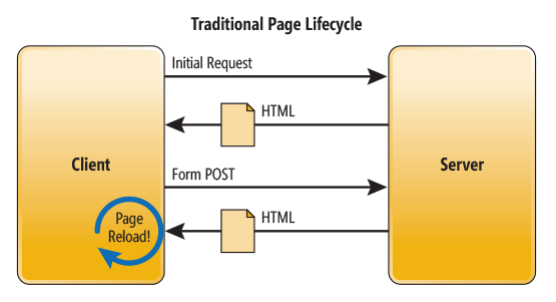
\includegraphics[width=0.6\linewidth]{traditional_lifecycle}

\section{SPA Overview}

\begin{minipage}[c]{.6\linewidth}
    \begin{itemize}
        \item Plain HTML/CSS/JS Code \\(no plugin)
        \item No page reloads
        \item Working back button
        \item Bookmarkable Links
        \item (limited) offline functionality
        \item Uses RESTful Services \\for data access
    \end{itemize}
\end{minipage}%
\begin{minipage}[c]{.4\linewidth}
    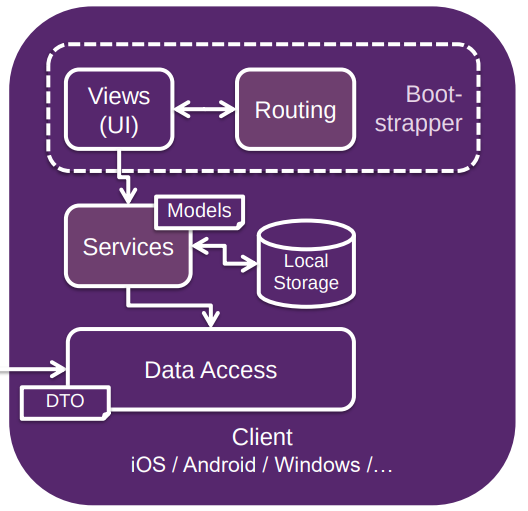
\includegraphics[width=\linewidth]{spa_arch}
\end{minipage}%
\\ % important

\subsection{Routing}
Browser fakes the URL change.
\\
Use \textbf{Anchors \#} or \textbf{window.history} API

\subsection{Bundling with WebPack}
\begin{description}
    \item[Entry] Startpunkt wo Webpack mit Bundling beginnt und
    Dependencies findet.
    \item[Output] Where to bundle your application.
    \item[Loaders] Transformiert Dateien in Module. (\textit{module})
    \item[Mode] Enable built-in \textit{optimization} mechanisms.
\end{description}

% TODO probably move me somewhere else when we get to Angular. Or remove me completely
\subsection{Dependency Injection}
\begin{itemize}
    \item Reduced coupling between consumer and impl.
    \item Classes relate to each other not directly but by interfaces
    \item Allows flexible replacement of implementation
\end{itemize}

\section{React}

\subsection{JSX}
JSX wird vom Präprozessor zu \mintinline{jsx}|React.createElement| Aufrufen umgewandelt => React import nötig!
\begin{minted}{jsx}
import React from 'react'

const menu = entries.map(entry =>
  <ListItem as="a" to={`/${entry.path}`}>
    <h1>{entry.title.toUpperCase()}</h1>
    <p className="lg">{entry.subtitle}</p>
  </ListItem>
)
\end{minted}

\subsubsection{Conditionals}
\begin{minted}{jsx}
{ error &&
    <Message>Fehler: {error}</Message> }
{ error ? <span>Fehler: {error}</span>
        : <span>OK!</span>             }
\end{minted}

\subsubsection{Function \& Const}
\begin{minted}{jsx}
function HelloMessage(props) {
  return <div>Hello {props.name}</div>;
}
const HelloMessage =
  (props) => <div>Hello {props.name}</div>;
\end{minted}

\subsection{Mounting}
Komponenten müssen gemounted werden damit diese angezeigt werden können.
\begin{minted}{jsx}
const root = ReactDOM.createRoot(
  document.getElementById('root'));
root.render(<App />);
\end{minted}

\subsection{Props}
Alle Parameter sind in \textbf{props} Objekt. Read-only!

\subsection{State}
\begin{itemize}
    \item \textbf{useState} immer in derselben Reihenfolge aufrufen!
    \item Keine von Props abgeleiteten Daten im State!
    \item Props bevorzugen!
\end{itemize}

\begin{minted}{jsx}
const [value, setValue] = useState(0);
const increment =
  () => setCounter(counter + 1);
return
  <button onClick={increment}>Inc</button>
\end{minted}

Weiter ab Reat Folie 44

\section{Angular}

\section{ASP.NET}

\end{multicols*}
\end{document}